\documentclass[aspectratio=169,xcolor=table]{beamer}
%aspcetratio >> 1610 169 149 54 43 32
%The themes:
\usetheme[style=classic]{mharvellous}
% \usetheme[style=dark]{mharvellous}
% \usetheme[style=mracula]{mharvellous}
% \usetheme[style=default]{mharvellous}
%*--------------------------------------------------
%\usepackage{helvet}
%*--------------------------------------------------
\usepackage{bibunits}
%\setbeamertemplate{bibliography item}{[\theenumiv]}
\setbeamertemplate{bibliography item}{\insertbiblabel}
\defaultbibliography{bibliography}
%\defaultbibliographystyle{IEEEtran}
%\defaultbibliographystyle{amsalpha}
\defaultbibliographystyle{abntex2-alf}
%\bibliography{bibliography}
%\usepackage[backend=biber,style=alphabetic,citestyle=authoryear]{biblatex}
% \addbibresource{bibliography.bib}
%\usepackage{natbib}
\usepackage{bibentry}
%*--------------------------------------------------
\usepackage{lipsum}
\usepackage{epigraph}
\usepackage{graphicx}
\usepackage{multirow}
%\usepackage{enumitem}
\usepackage{array}
%\usepackage{multimedia}
\usepackage{media9}
%\usepackage{pdfpc-movie}
\usepackage{circledsteps}
\usepackage{listings}
\usepackage[normalem]{ulem}
%\usepackage{Sweave}
%\usepackage{xkeyval}
%\usepackage{palatino}
%\usepackage{pgfpages}
\usepackage{float}
%*--------------------------------------------------
\usepackage{subcaption} % sub imagem nas figuras
\usepackage{lmodern}
%*--------------------------------------------------
\usepackage[timeinterval=1]{tdclock}
%\usepackage[font=Times,timeinterval=1, timeduration=200,resetatpages=all]{tdclock}
%\usepackage[font=Times,timeinterval=10, timeduration=2.0, timedeath=0, fillcolorwarningsecond=white!60!yellow,timewarningfirst=50,timewarningsecond=80,resetatpages=2]{tdclock}
%*--------------------------------------------------
\usepackage{url}
\usepackage{tabularx,booktabs}
\usepackage{threeparttable}
\usepackage[absolute, overlay]{textpos}
%*--------------------------------------------------
\usepackage{framed, color}
\usepackage[tikz]{bclogo}
\usepackage{spot}
\setspotlightcolor{red!50}
% %\setspotlightstyle{star, fill=red!50}
% %\setspotlightstyle{star points=7}
\usepackage{color,soul}
%\usepackage{xcolor}
\usepackage{tcolorbox}
\usepackage{xcolor}
\usepackage[export]{adjustbox}
\usepackage{verbatim}
\usetikzlibrary{trees,shapes,arrows}
\usepackage{fancyvrb}
\usepackage{float}
%*--------------------------------------------------
\usepackage{amsmath}
\usepackage{xfrac}
\usepackage{units}
\usepackage{ulem}
%*-------------------------------------------------------------------------------
%\newcolumntype{C}[1]{>{\centering\arraybackslash}m{#1}}
\newcolumntype{L}[1]{>{\raggedright\let\newline\\\arraybackslash\hspace{0pt}}m{#1}}
\newcolumntype{C}[1]{>{\centering\let\newline\\\arraybackslash\hspace{0pt}}m{#1}}
\newcolumntype{R}[1]{>{\raggedleft\let\newline\\\arraybackslash\hspace{0pt}}m{#1}}
%*-------------------------------------------------------------------------------
%\pgfpagesuselayout{2 on 1}[a4paper,border shrink=5mm]
%\setbeamertemplate{note page}[plain]
%\setbeameroption{show notes on second screen=bottom}
%*-------------------------------------------------------------------------------
\setbeameroption{hide notes}
%\setbeameroption{show only notes}
%\setbeameroption{show notes on second screen=right}
\setbeamertemplate{note page}{\pagecolor{yellow!5}\insertnote}
%*-------------------------------------------------------------------------------

%*-------------------------------------------------------------------------------
\title              {Article presentation}
\subtitle           {Dynamical Models For Omni-Directional Robots With 3 And 4 Wheels}
\author             {Erick Suzart Souza}
\email              {ericksuzart@gmail.com}
\advisor            {Orientador: Marco A. dos Reis}
\institute          {Robótica e Sistemas Autônomos, Senai Cimatec}
\date               {Abril de 2022}
% \ulogo        		{Template/logosenaicimatecnegativo}
% \ulogof             {Template/logosenaicimatec2020}
% \ulogoo        		{Template/rosa-logo}
% \ulistelement    	{Template/bullet-white}

%*-------------------------------------------------------------------------------
\graphicspath{{Source/pictures/}}
%*-------------------------------------------------------------------------------
\totalNoSlidesDisabled % To turn off the total number of slides in the footer. Comment this if you want the total number of slides in the footer
%*-------------------------------------------------------------------------------
\begin{document}
  %*----------- COVER -------------------------------------------------------------
  \begin{frame}[t,plain]
    %*----------- sound--------------------------------
    % \includemedia[
    %   %width=1ex,
    %   %height=1ex,
    %   %activate=pageopen, 
    %   activate=onclick,
    %   deactivate=onclick,
    %   %passcontext,
    %   transparent,
    %   addresource=./Source/sounds/hip-hop.mp3,
    %   flashvars={
    %     source=./Source/sounds/hip-hop.mp3
    %     %&autoPlay=true
    %     &autoRewind=true
    %     &Play=2s
    %     &repeat=always
    %     %&Loop=true
    %   }
    % ]
    % {}{VPlayer.swf}
    %*----------- start-page--------------------------
    \titlepage
    %*----------- notes-------------------------------
    \note[item]{Notes can help you to remember important information. Turn on the notes option.}
  \end{frame}
  %-
  %*----------- SECTIONS ----------------------------------------------------------
  

%*----------- SLIDE -------------------------------------------------------------
\begin{frame}[c]{Objetivo}
  \framesubtitle{Da apresentação}
  \transdissolve[duration=0.5]

  \begin{center}
    \Wider{
      \begin{shaded}
        \begin{center}
          \vspace*{0.5cm}
          \resizebox{!}{0.6cm}{%
            \color{black} Entendimento do artigo
          }
        \end{center}
      \end{shaded}
    }
  \end{center}


  %*----------- notes
  \note[item]{Notes can help you to remember important information. Turn on the notes option.}
\end{frame}

%-
%*----------- SLIDE -------------------------------------------------------------

\begin{frame}[t]{Introdução}
  \framesubtitle{O problema}
  \transdissolve[duration=0.5]
  Baixa precisão no comportamento do robô.

  \begin{columns}[t]
    \column{.6\linewidth}
      \begin{figure}
        \includemedia[
          totalheight=0.5\linewidth,
          activate=pageopen,
          passcontext,
          %transparent,
          addresource=./Source/gifs/atlas-jump.wmv,
          flashvars={
            source=./Source/gifs/atlas-jump.wmv
            &autoPlay=true
            &autoRewind=true
            &loop=true}
            ]{\fbox{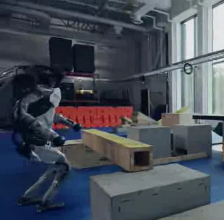
\includegraphics{Source/gifs/atlas-jump.png}}}{VPlayer.swf}
          \caption{Expectativa \cite{BostonDynamicsPartners}} %FIXME: slides não estão numerando as figuras
      \end{figure}
    \column{.6\linewidth}
    \begin{center}
      %\centerline{
      \begin{figure}
        \includemedia[
          totalheight=0.5\linewidth,
        activate=pageopen,
        passcontext,
        %transparent,
        addresource=./Source/gifs/atlas-fail.wmv,
        flashvars={
          source=./Source/gifs/atlas-fail.wmv
          &autoPlay=true
          &autoRewind=true
          &loop=true}
          ]{\fbox{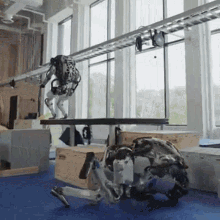
\includegraphics{Source/gifs/atlas-fail.png}}}{VPlayer.swf}
        \caption{Realidade \cite{BostonDynamicsFails}}
      \end{figure}
    \end{center}
  \end{columns}
  %*----------- notes
  \note[item]{Notes can help you to remember important information. Turn on the notes option.}
\end{frame}

%*----------- SLIDE -------------------------------------------------------------
\begin{frame}[t]{Introdução}
  \framesubtitle{O robô utilizado}
  \transdissolve[duration=0.5]

  \begin{figure}[ht!]
    \centering
    \begin{subfigure}[b]{0.3\textwidth}
      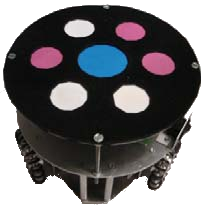
\includegraphics[width=\textwidth]{Three_wheeled_robot.png}
      % \roundpic[xshift=0cm,yshift=0cm]{4.5cm}{4.5cm}{Three_wheeled_robot.png}
      \caption{Três rodas.}
      \label{fig:3_wheels_robot}
    \end{subfigure}
    ~
    \begin{subfigure}[b]{0.3\textwidth}
      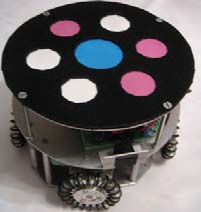
\includegraphics[width=\textwidth]{four_wheeled_robot.png}
      % \roundpic[xshift=0cm,yshift=0cm]{4.5cm}{4.5cm}{four_wheeled_robot.png}
      \caption{Quatro rodas.}
      \label{fig:4_wheels_robot}
    \end{subfigure}
    
  \caption{Plataforma utilizada para comparar às duas configurações. \cite{Oliveira2008}}
  \end{figure}
  
  %*----------- notes
  \note[item]{Notes can help you to remember important information. Turn on the notes option.}
\end{frame}

%-
%*----------- SLIDE -------------------------------------------------------------
\begin{frame}[t]{Introdução}
  \framesubtitle{As causas elencadas}
  \transdissolve[duration=0.5]
  \begin{enumerate}
    \item Modelo dinâmico incompleto.
    \begin{enumerate}
      \item Dificuldade em modelar os atritos internos.
    \end{enumerate}

    \item Parâmetros imprecisos (específico).
    \begin{enumerate}
      \item Coeficientes de atrito.
      \item Momento inercial.
      \item Constantes dos motores.
    \end{enumerate}
  \end{enumerate}

  %*----------- notes
  \note[item]{Notes can help you to remember important information. Turn on the notes option.}
\end{frame}

%*----------- SLIDE -------------------------------------------------------------
\begin{frame}[c]{Objetivo}
  \framesubtitle{Do artigo}
  \transdissolve[duration=0.5]

  \begin{center}
    \Wider{
      \begin{shaded}
        \begin{center}
          \vspace*{0.5cm}
          \resizebox{!}{0.6cm}{%
            \color{black} Encontrar um modelo dinâmico preciso
          }
        \end{center}
      \end{shaded}
    }
  \end{center}


  %*----------- notes
  \note[item]{Notes can help you to remember important information. Turn on the notes option.}
\end{frame}

  
%*----------- SLIDE -------------------------------------------------------------
\begin{frame}[t]{A abordagem}
  \transboxout[duration=0.5]
  \framesubtitle{Diagrama}

  % Define block styles
  \tikzstyle{decision} = [diamond, draw, fill=blue!20,
  text width=4.5em, text badly centered, node distance=3cm, inner sep=0pt]
  \tikzstyle{block} = [rectangle, draw, fill=blue!20,
  text width=5em, text centered, rounded corners, minimum height=4em, node distance=3cm]
  \tikzstyle{line} = [draw, -latex']
  \tikzstyle{cloud} = [draw, ellipse,fill=red!20, node distance=3cm,
  minimum height=2em]

  \begin{center}
    \begin{tikzpicture}[node distance = 2cm, auto]
      % Place nodes
      \node [block] (mec) {Estrutura Mecânica};
      \node [block, right of=mec] (kinematic) {Modelo Cinemático};
      \node [block, right of=kinematic] (dynamic) {Modelo Dinâmico};
      \node [block, right of=dynamic] (param) {Estimativa dos Parâmetros};
  
      % \node [cloud, left of=mec] (init) {init};
      % \node [block, below of=init] (identify) {identify candidate models};
      % \node [block, below of=identify] (evaluate) {evaluate candidate models};
      % \node [block, left of=evaluate, node distance=3cm] (update) {update model};
      % \node [decision, below of=evaluate] (decide) {is best candidate better?};
      % \node [block, below of=decide, node distance=3cm] (stop) {stop};
  
      % Draw edges
      \path [line] (mec) -- (kinematic);
      \path [line] (kinematic) -- (dynamic);
      \path [line] (dynamic) -- (param);
      % \path [line] (evaluate) -- (decide);
      % \path [line] (decide) -| node [near start] {yes} (update);
      % \path [line] (update) |- (identify);
      % \path [line] (decide) -- node {no}(stop);
      % \path [line] (system) -- (init);
      % \path [line,dashed] (system) |- (evaluate);
    \end{tikzpicture}
  \end{center}

  %*----------- notes
  \note[item]{Notes can help you to remember important information. Turn on the notes option.}
\end{frame}

%*----------- SLIDE -------------------------------------------------------------
\begin{frame}[c]{A abordagem}
  \framesubtitle{Estrutura Mecânica}
  \transdissolve[duration=0.5]

  \begin{figure}[ht!]
    \centering
    \begin{subfigure}[b]{0.38\textwidth}
      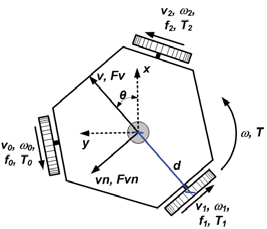
\includegraphics[width=\textwidth]{three_wheeled_robot_geometry.png}
      \caption{Três rodas.}
      \label{fig:3_wheels_robot_geometry}
    \end{subfigure}
    ~
    \begin{subfigure}[b]{0.38\textwidth}
      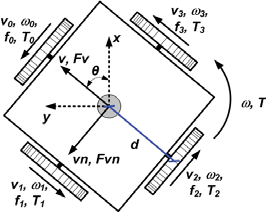
\includegraphics[width=\textwidth]{four_wheeled_robot_geometry.png}
      \caption{Quatro rodas.}
      \label{fig:4_wheels_robot_geometry}
    \end{subfigure}
    
    \caption{Estrutura geométrica de ambas as configurações do robô. \cite{Oliveira2008}}
  \end{figure}


  %*----------- notes
  \note[item]{Notes can help you to remember important information. Turn on the notes option.}
\end{frame}

%*----------- SLIDE -------------------------------------------------------------
\begin{frame}[c]{A abordagem}
  \framesubtitle{Modelo Cinemático}
  \transdissolve[duration=0.5]

    


  %*----------- notes
  \note[item]{Notes can help you to remember important information. Turn on the notes option.}
\end{frame}


{
  \setbeamertemplate{background}
  {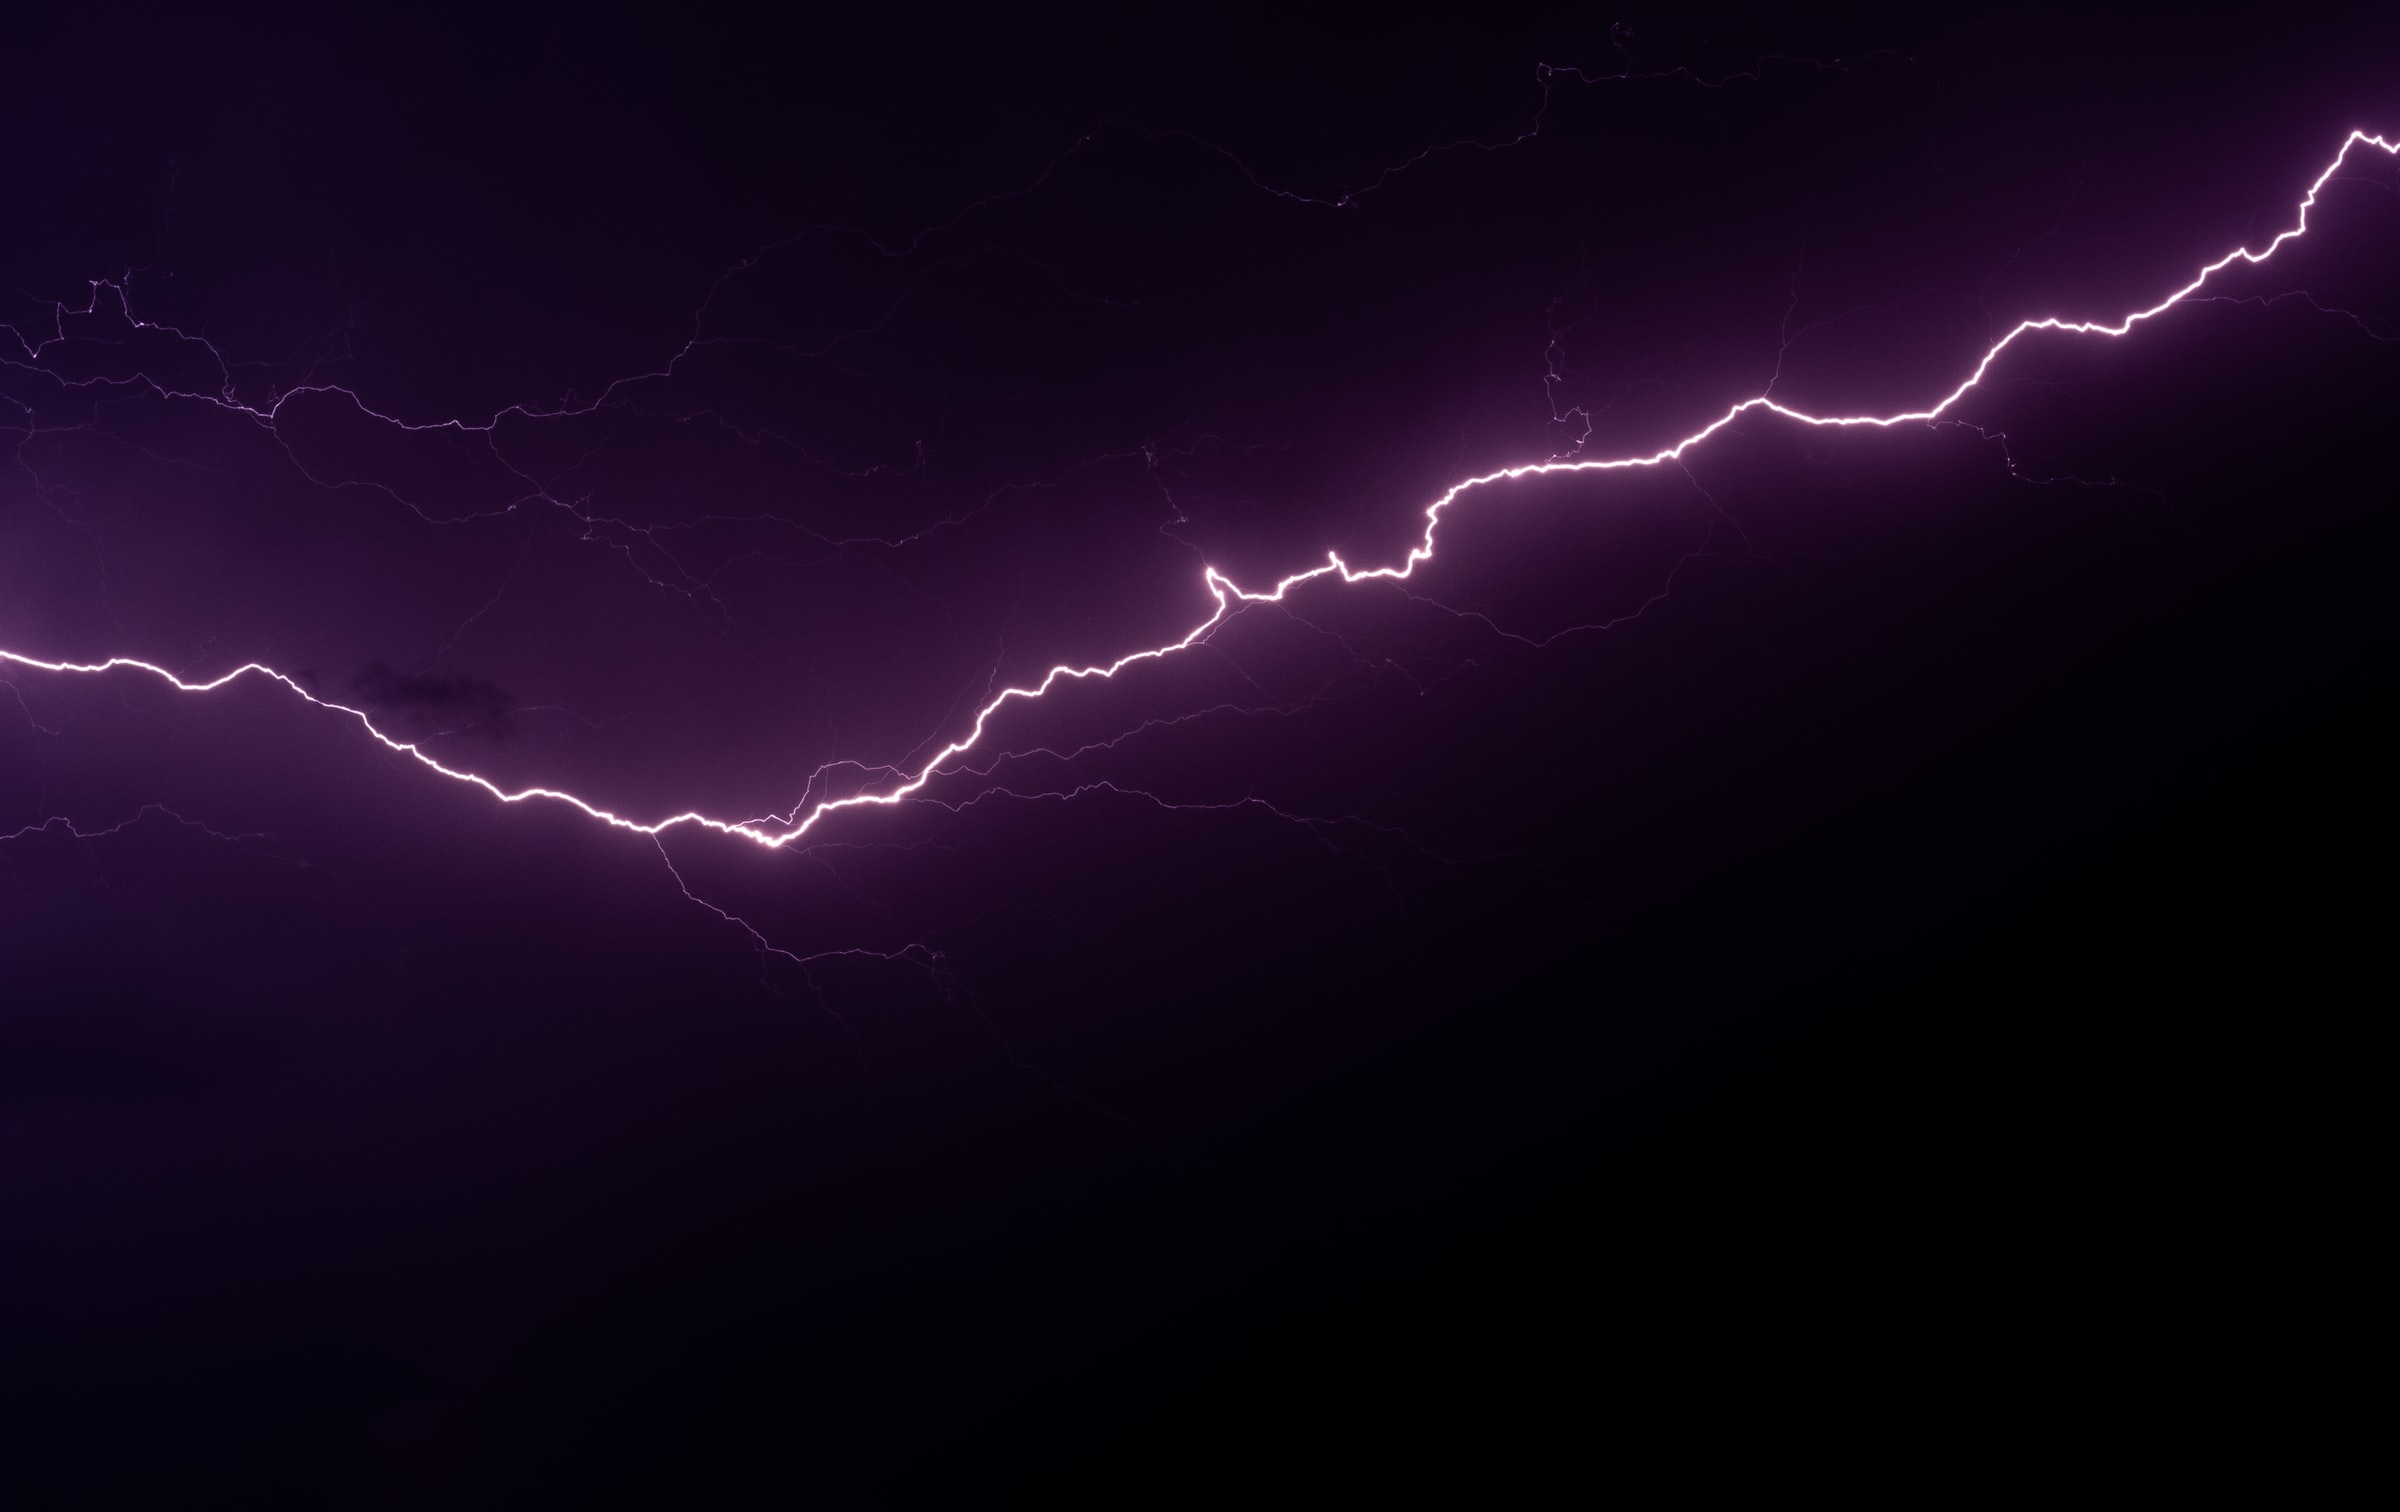
\includegraphics[trim = 0 0 0 0, clip, width = \the\paperwidth, height = \the\paperheight]{marcel-knupfer-37wuETxVwTQ-unsplash.jpg}}
  %*----------- SLIDE -------------------------------------------------------------
  \begin{frame}[c]{}
    \transboxout[duration=0.5]

    \begin{columns}
      \column{.1\textwidth}
      \column{.3\textwidth}
      \column{.53\textwidth}
      \vspace*{-3.5cm}
      \Huge{\textbf{\textcolor{mracula5}{Quando chovia...}}}
    \end{columns}
    %*----------- notes
    \note[item]{Notes can help you to remember important information. Turn on the notes option.}
  \end{frame}
  %-
}
%*----------- SLIDE -------------------------------------------------------------
\begin{frame}[t]{O sistema robótico}
  \transboxout[duration=0.5]
  \framesubtitle{Darwin-OP}
  \begin{columns}
    \column{.1\textwidth}
    \column{.4\textwidth}
    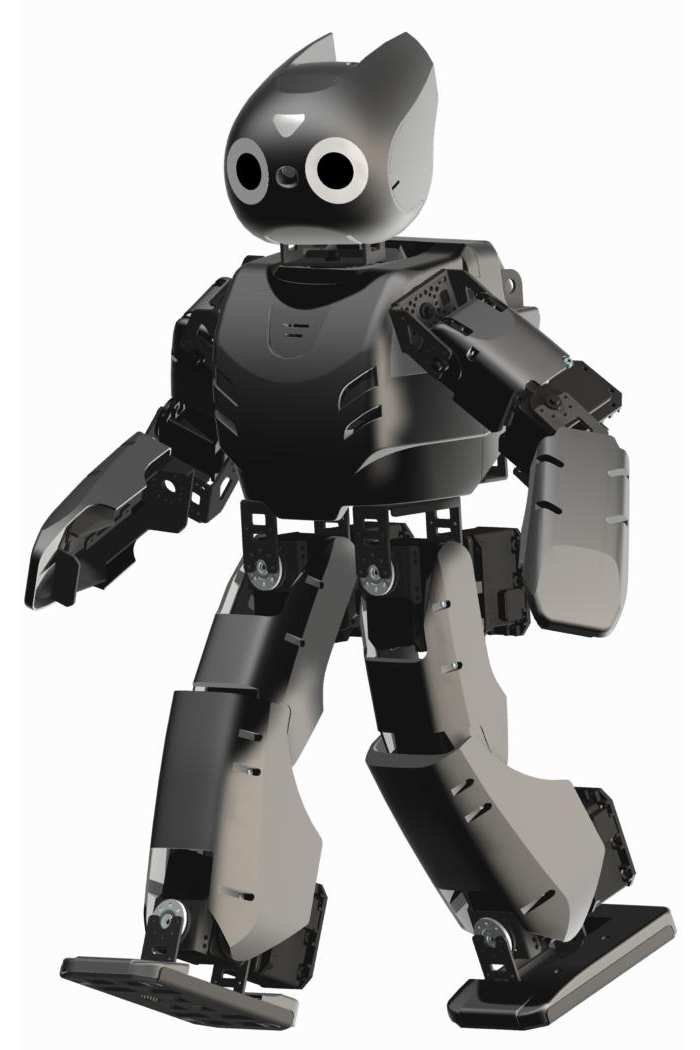
\includegraphics[width=.7\textwidth]{darwin-op}
    \column{.4\textwidth}
    \begin{enumerate}
      \item plataforma antropormórfica Darwin-OP;
      \item 20 DoF\footnote{do inglês, graus de liberdade};
      \item composto de 18 servo-motores;
      \item possui um grande gama de sensores para interação.
    \end{enumerate}
  \end{columns}
  %*----------- notes
  \note[item]{Notes can help you to remember important information. Turn on the notes option.}
\end{frame}
%-
%*----------- SLIDE -------------------------------------------------------------
\begin{frame}[c]{Darwin-OP - overview}
  %\transboxin[duration=1,direction=30]
  \centering

  \includemedia[
  width=0.7\linewidth,
  totalheight=0.39375\linewidth,
  activate=pageopen,
  passcontext,
  addresource=./Source/movies/Darwin-OP.mp4,
  flashvars={
    source=./Source/movies/Darwin-OP.mp4
    &autoPlay=true
    &Loop=false}
  ]{\fbox{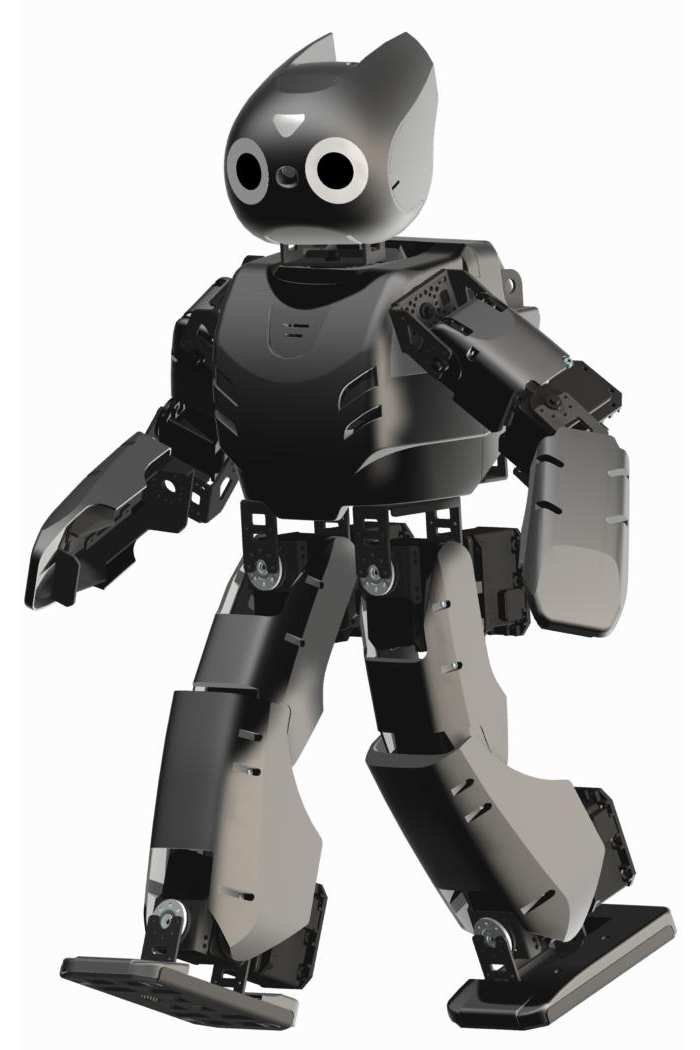
\includegraphics{darwin-op}}}{VPlayer.swf}

  %*----------- notes
  \note[item]{Notes can help you to remember important information. Turn on the notes option.}
\end{frame}
%-
%*----------- SLIDE -------------------------------------------------------------
\begin{frame}[t]{O sistema robótico}
  \transboxout[duration=0.5]
  \framesubtitle{Darwin-OP}
  \begin{columns}
    \column{.1\textwidth}
    \column{.4\textwidth}
    \column{.4\textwidth}
  \end{columns}

  \begin{block}{Um bloco de destaque}
    Um exemplo de block.\\
    Oferece um certo destaque.
  \end{block}

  \begin{alertblock}{Um bloco de destaque}
    Um exemplo de alertblock.\\
    Oferece um certo destaque.
  \end{alertblock}

  \begin{exampleblock}{Um bloco de destaque}
    Um exemplo de exampleblock.
  \end{exampleblock}
  %*----------- notes
  \note[item]{Notes can help you to remember important information. Turn on the notes option.}
\end{frame}
%-
%*----------- SLIDE -------------------------------------------------------------
\begin{frame}[t]{O sistema robótico}
  \transboxout[duration=0.5]
  \framesubtitle{PlantUML}

  \tikzstyle{every node}=[draw=black,thick,anchor=west]
  \tikzstyle{selected}=[draw=red,fill=red!30]
  \tikzstyle{optional}=[dashed,fill=gray!50]

  \begin{tikzpicture}[%
    grow via three points={one child at (0.5,-0.7) and
      two children at (0.5,-0.7) and (0.5,-1.4)},
    edge from parent path={(\tikzparentnode.south) |- (\tikzchildnode.west)}]
    \node {texmf}
    child { node {doc}}
    child { node {fonts}}
    child { node {source}}
    child { node [selected] {tex}
      child { node {generic}}
      child { node [optional] {latex}}
      child { node {plain}}
    }
    child [missing] {}
    child [missing] {}
    child [missing] {}
    child { node {texdoc}};
  \end{tikzpicture}

  %*----------- notes
  \note[item]{Notes can help you to remember important information. Turn on the notes option.}
\end{frame}
%-
%*----------- SLIDE -------------------------------------------------------------
\begin{frame}[t]{O sistema robótico}
  \transboxout[duration=0.5]
  \framesubtitle{PlantUML}

  % Define block styles
  \tikzstyle{decision} = [diamond, draw, fill=blue!20,
  text width=4.5em, text badly centered, node distance=3cm, inner sep=0pt]
  \tikzstyle{block} = [rectangle, draw, fill=blue!20,
  text width=5em, text centered, rounded corners, minimum height=4em]
  \tikzstyle{line} = [draw, -latex']
  \tikzstyle{cloud} = [draw, ellipse,fill=red!20, node distance=3cm,
  minimum height=2em]

  \begin{tikzpicture}[node distance = 2cm, auto]
    % Place nodes
    \node [block] (init) {initialize model};
    \node [cloud, left of=init] (expert) {expert};
    \node [cloud, right of=init] (system) {system};
    \node [block, below of=init] (identify) {identify candidate models};
    \node [block, below of=identify] (evaluate) {evaluate candidate models};
    \node [block, left of=evaluate, node distance=3cm] (update) {update model};
    \node [decision, below of=evaluate] (decide) {is best candidate better?};
    \node [block, below of=decide, node distance=3cm] (stop) {stop};
    % Draw edges
    \path [line] (init) -- (identify);
    \path [line] (identify) -- (evaluate);
    \path [line] (evaluate) -- (decide);
    \path [line] (decide) -| node [near start] {yes} (update);
    \path [line] (update) |- (identify);
    \path [line] (decide) -- node {no}(stop);
    \path [line,dashed] (expert) -- (init);
    \path [line,dashed] (system) -- (init);
    \path [line,dashed] (system) |- (evaluate);
  \end{tikzpicture}

  %*----------- notes
  \note[item]{Notes can help you to remember important information. Turn on the notes option.}
\end{frame}
%-
%*----------- SLIDE -------------------------------------------------------------
\begin{frame}[t]{O sistema robótico}
  \transboxout[duration=0.5]
  \framesubtitle{PlantUML}

  \begin{tikzpicture}[line width=0.1pt]
    \draw(0,0) circle(5cm);
    \draw(0,0) circle(1cm);
    \draw(0,0) node {\Huge$\mathbf{A}$};
    \draw(0,0) circle(4.5cm);
    \draw(-48:2.5) arc(-48:240:2.5cm);
    %% The outer nodes
    \foreach \x in {36,72,...,360}
    \shade[ball color=black](\x:5) circle(4pt);
    \foreach \nodes in {12,24,...,360}
    \shade[ball color=black](\nodes:3.5) circle(4pt);
    %%% The connecting nodes
    \foreach \angle in {-48,-12,...,240}
    \draw(\angle:2.5) --++(\angle:0.9cm);
    %%% outer interconnects
    \foreach \angle in {-24,12,...,306}
    \draw(\angle:3.6) --++(\angle:0.9cm);
    \foreach \y in {-24,12,...,240}
    \shade[ball color=black](\y:4.5cm) circle(4pt);

    %% outer most connections
    \foreach \angle in{-36,0,...,306}
    \draw(\angle:4.9cm) --(\angle:4.7cm) [rotate=\angle]arc(0:180:0.20cm);
    \foreach \angle in{-36,0,...,306}
    \draw(\angle:4.3cm) --(\angle:3.6cm);
    %% Outer connects and leads
    \shade[ball color=black](276:6) circle(4pt);
    \draw(276:6)circle(4pt)--(276:5.2)[rotate=276]arc(0:180:0.25cm);
    \draw(276:7)node {$\mathbf{K_0}$};
    \draw(276:4.2)[rotate=276]arc(180:360:0.25cm);
    \draw(276:4.2)--(276:3.5);

    %% Exploitation of circular symmetry of the required figure

    {[rotate=72]
      \shade[ball color=black](276:6) circle(4pt);
      \draw(276:6)circle(4pt)--(276:5.2)[rotate=276]arc(0:180:0.25cm);
      \draw(270:6)node {$\mathbf{K_1-K_9}$};
      \draw(276:4.2)[rotate=276]arc(180:360:0.25cm);%%%
      \draw(276:4.2)--(276:3.5);
    }

    {[rotate=-48]
      \shade[ball color=black](276:6) circle(4pt);
      \draw(276:6)circle(4pt)--(276:5.2)[rotate=276]arc(0:180:0.20cm);
      \draw(276:7)node {$\mathbf{g_2}$};
      \draw(276:4.8)--(276:4.5);
    }

    \draw(180:5)--(180:6);
    \shade[ball color=black](180:6) circle(4pt);
    \draw(180:6.5)node{$\mathbf{g_1}$};
  \end{tikzpicture}

  %*----------- notes
  \note[item]{Notes can help you to remember important information. Turn on the notes option.}
\end{frame}
%-

%*----------- SLIDE -------------------------------------------------------------
\begin{frame}[c]{A tropa dos quatro incríveis}
  %\transboxin[duration=1,direction=30]
  A simulação deverá ser desenvolvida com 4 unidades Darwin-OP, comumente esta unidade é utilizada para desafios em competições de robótica.
  \newline

  A tropa será composta por 4 Darwin-OP, e deverá realizar duas missões:
  \begin{itemize}
      \item marchar em forma unida em linha;
      \item realizar corrida de revezamento.
  \end{itemize}

  \begin{figure}
      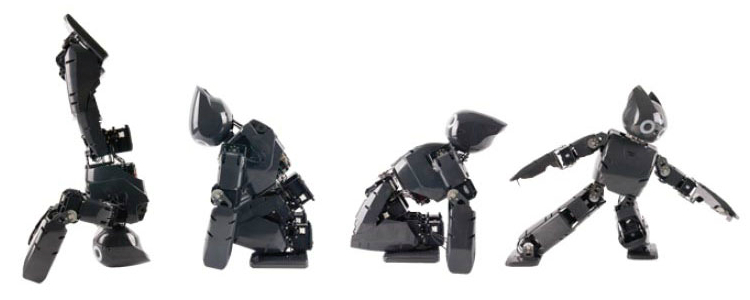
\includegraphics[trim = 0 20 0 50, clip, width=0.8\textwidth]{darwin-op-sequencia}
      %\caption{.}
  \end{figure}
%*----------- notes
  \note[item]{Notes can help you to remember important information. Turn on the notes option.}
\end{frame}
%-
%*----------- SLIDE -------------------------------------------------------------
\begin{frame}[t]{Algumas regras}
  \begin{itemize}
      \item A marcha deverá ser realizada diante de um percurso de 2 metros.
      \item A marcha e a corrida de revezamento deverão serem realizadas numa pista de corrida;
      \item A corrida deverá ser realizada numa pista de 8 metros;
      \item Cada Darwin-OP deverá percorrer 2 metros para realizar o revezamento;
      \item A região de revezamento deverá ser uma área de até 0.4 metros;
      \item O conceito para o revezamento será o de alinhar-se os dois Darwin-OP durante até 15 segundos a uma distância de no máximo 0.2 metros entre ambos, ou seja será considerado passagem de bastão quando os dois Darwin-OP passarem 15 segundos com movimentos sincronizados a uma distância máxima de 0.2 metros dentro da região de revezamento;
      \item A pista de corrida deverá ser considerada analogamente a uma pista real;
      \item A lateral da pista deverá ter lados de 2 metros;
      \item Considerar sempre os critérios de uma corrida de revezamento.
  \end{itemize}
  
  % \begin{columns}[t]
  %     \column{.45\textwidth}
  %         detalhar sistemas em subconjuntos\\
  %         listar possíveis modos de falhas\\
  %         analisar cada modo de falha, juntamente com suas possíveis causas e sintomas
  %     \column{.45\textwidth}
  %         estimar os efeitos de cada modo de falhas\\
  %         estimar a criticidade de cada efeito\\
  %         identificar ações para minimizar falhas
  % \end{columns}
%*----------- notes
  \note[item]{Notes can help you to remember important information. Turn on the notes option.}
\end{frame}
%-
%*----------- SLIDE -------------------------------------------------------------
\begin{frame}[c]{A pista}
  \begin{figure}
      %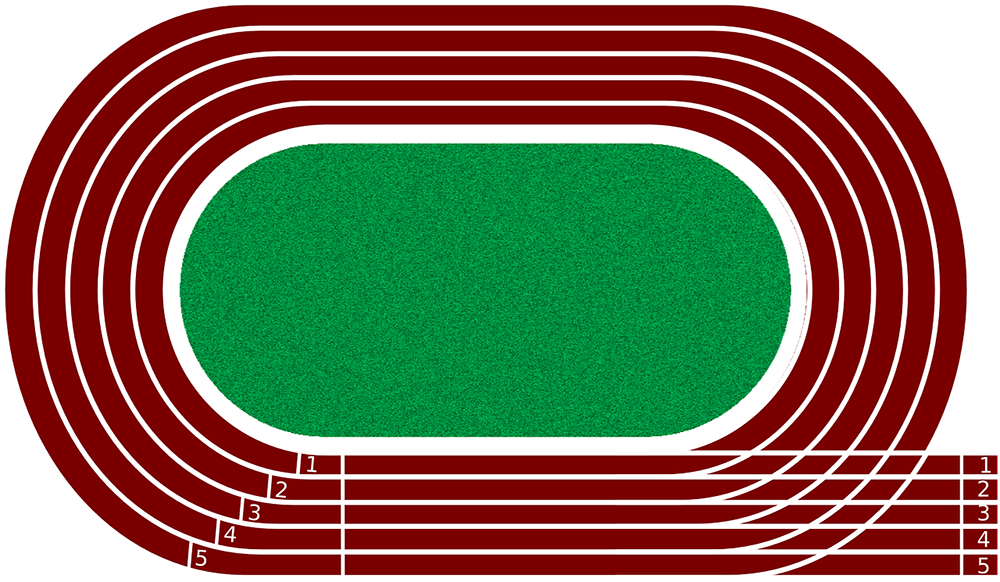
\includegraphics[width=0.7\textwidth]{pista_corrida}
      
      \roundpic[xshift=0cm,yshift=0cm]{3cm}{7cm}{pista_corrida}
        
      \caption{Formato de um pista de corrida.\cite{agostini2007}}
  \end{figure}
%*----------- notes
  \note[item]{Notes can help you to remember important information. Turn on the notes option.}
\end{frame}
%-
  %-
%*----------- SLIDE -------------------------------------------------------------
\begin{frame}[t]{Resultados}
    \transdissolve[duration=0.5]
    % \begin{table}
    %   \begin{tabular}{ c c c }
    %     Parameters           &	 3 wheels  &  4 wheels \\
    %     d (m)                &   0.0       &  89       \\
    %     r (m)                &   0.0       &  325      \\ 
    %     l                    &             &  5        \\
    %     $K_v (V /(rad/s))$ &   0.0       &  259      \\
    %     R (Ω)                &   4.3       &  111      \\
    %     M (kg)               &   1.944     &  2.34     \\
    %     J (kg · m2 )         &   0.0169    &  0.0228   \\
    %     $B_v (N/(m/s))$    &   0.5082    &  0.4978   \\
    %     $B_{vn} (N/(m/s))$ &   0.4870    &  0.6763   \\
    %     $B_ω (N · m/(rad/s))$ &0.0130    &  0.0141   \\
    %     $C_v (N)$          &   1.9068    &  1.8738   \\
    %     $C_{vn} (N)$       &   2.0423    &  2.2198   \\
    %     $C_ω (N · m)$      &   0.0971    &  0.1385 
    %   \end{tabular}
    % \end{table}
    \begin{figure}[ht!]
      \centering
  
      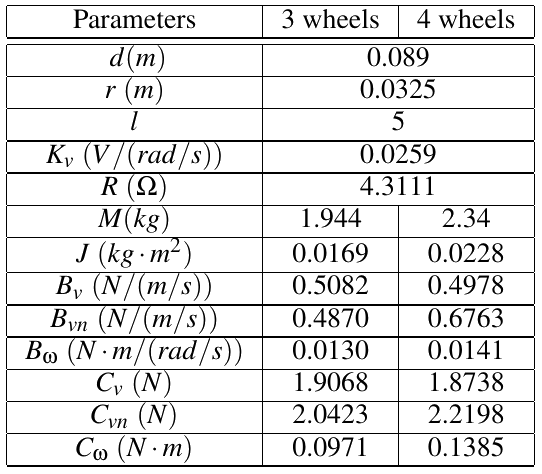
\includegraphics[width=0.9\textheight]{table.png}
      \label{fig:result_table}
  
    \end{figure}
  
    %*----------- notes
    \note[item]{Notes can help you to remember important information. Turn on the notes option.}
  \end{frame}


%*----------- SLIDE -------------------------------------------------------------
\begin{frame}[t]{Resultados}
  \transdissolve[duration=0.5]

  \begin{figure}[ht!]
    \centering
    \begin{subfigure}[b]{0.4\textwidth}
      \centering
      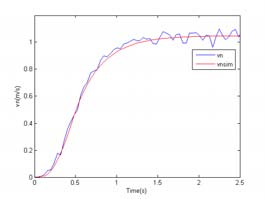
\includegraphics[width=\textwidth]{result_graph_3w_vn.png}
      % \roundpic[xshift=0cm,yshift=0cm]{4.5cm}{4.5cm}{Three_wheeled_robot.png}
      \caption{Velocidade no eixo vn.}
      \label{fig:result_3w_vn}
    \end{subfigure}
    ~
    \begin{subfigure}[b]{0.4\textwidth}
      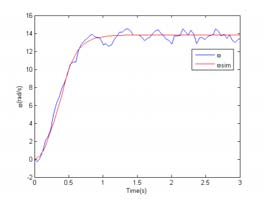
\includegraphics[width=\textwidth]{result_graph_3w_w.png}
      % \roundpic[xshift=0cm,yshift=0cm]{4.5cm}{4.5cm}{four_wheeled_robot.png}
      \caption{Velocidade em rotação.}
      \label{fig:result_3w_w}
    \end{subfigure}    
  \caption{Validação do modelo (3 rodas).}
  \end{figure}
  
  %*----------- notes
  \note[item]{Notes can help you to remember important information. Turn on the notes option.}
\end{frame}

%*----------- SLIDE -------------------------------------------------------------
\begin{frame}[t]{Resultados}
  \transdissolve[duration=0.5]

  \begin{figure}[ht!]
    \centering
    \begin{subfigure}[b]{0.4\textwidth}
      \centering
      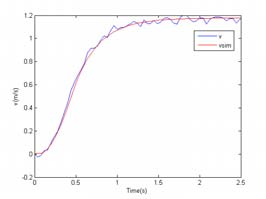
\includegraphics[width=\textwidth]{result_graph_4w_v.png}
      % \roundpic[xshift=0cm,yshift=0cm]{4.5cm}{4.5cm}{Three_wheeled_robot.png}
      \caption{Velocidade no eixo v.}
      \label{fig:result_4w_v}
    \end{subfigure}
    ~
    \begin{subfigure}[b]{0.4\textwidth}
      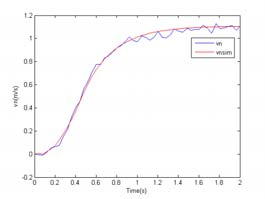
\includegraphics[width=\textwidth]{result_graph_4w_vn.png}
      % \roundpic[xshift=0cm,yshift=0cm]{4.5cm}{4.5cm}{four_wheeled_robot.png}
      \caption{Velocidade no eixo vn.}
      \label{fig:result_4w_vn}
    \end{subfigure}    
  \caption{Validação do modelo (4 rodas).}
  \end{figure}
  
  %*----------- notes
  \note[item]{Notes can help you to remember important information. Turn on the notes option.}
\end{frame}
  %-
%*----------- SLIDE -------------------------------------------------------------
\begin{frame}[t]{Finalmentes}
    \transdissolve[duration=0.5]
    \begin{enumerate}
      \item O modelo elaborado não considera derrapagem.
      \item Depende da construção do robô e seu peso.
      \item Estimativa dos parâmetros dependente dos experimentos.
      \item Outras abordagens?
    \end{enumerate}
  
    %*----------- notes
    \note[item]{Notes can help you to remember important information. Turn on the notes option.}
\end{frame}
  %----------------------------------------------------SLIDE------------------
 \begin{frame}[t, allowframebreaks]{References}
 %\frametitle{References}
%\begin{frame}{Reference}
    %\transboxin[duration=1,direction=30]

    % \begin{bibunit}[plain]
    % \cite{guangyi2018research}.
    % %\cite{kanakia2012}
    % %\cite{agostini2007}
    % %\cite{azuma1997survey}
    % \cite{Buss2005}
  
    % \putbib
    % \end{bibunit}
  
    %\bibliographystyle{IEEEtran}
    %\bibliographystyle{IEEEtranS}
    %\bibliographystyle{IEEEbib}
    \bibliographystyle{abntex2-alf}
    %\bibliographystyle{abntex2-num}
    %\bibliographystyle{abnt-alf}
    \bibliography{bibliography} 
    %\putbib

%*----------- notes
    %\note[item]{Notes can help you to remember important information. Turn on the notes option.}
\end{frame}
%
  %-
  %*----------- SLIDE-BACKUP ------------------------------------------------------
  % \backupbegin
  % %
  % \begin{frame}{Backup}
    %     Test
    % %*----------- notes-------------------------------
    % \note{Notes can help you to remember important information. Turn on the notes option.}
    % \end{frame}
  % %-
  % \backupend
  % %-
  %*----------- QUESTIONS ---------------------------------------------------------
  \begin{frame}[c,plain]
    \lastpage{
      \begin{center}   
        {\usebeamerfont{title} Questions?}\\[3ex] 
        %\hspace{1.5cm} 
        ericksuzart@gmail.com
      \end{center}
    }
    
    %*----------- notes---------------------------------
    \note[item]{Notes can help you to remember important information. Turn on the notes option.}
  \end{frame}
  %*-------------------------------------------------------------------------------
\end{document}